\section{نت‌کت پویا}
نک‌کت‌ پویا
\lf{DyNetKAT}
برای رفع برخی از کاستی‌های نت‌کت ارائه شده است
\cite{dynetkat}.
به صورت دقیق‌تر نت‌کت پویا، امکان توصیف به‌روز‌رسانی سیاست‌های شبکه و همچنین رفتار شبکه در مقابل چندین بسته را ممکن می‌سازد.

\subsection{دستور زبان نت‌کت پویا}
در نت‌کت‌ پویا، از رفتار انتها به انتها‌ی توصیف‌های شبکه در قالب عبارت‌های نت‌کت استفاده می‌شود.
به همین منظور سینتکس نت‌کت‌ پویا به صورت زیر تعریف می‌شود:
\begin{align*}
    N & :: = \mathrm{NetKAT}^{-dup}                    \\
    D & :: = \bot | N;D | x?N;D | x!N;D | D\parallel D
    D \oplus D | X                                     \\
      & X \triangleq D
\end{align*}
در سینتکس بالا
$\mathrm{NetKAT}^{-dup}$
قسمتی از زبان نت‌کت است که عبارت‌های
$dup$
از آن حذف شده است.
عبارت‌های
$dup$
در توصیف‌های نت‌کت تاثیری در رفتار یک عبارت ندارند و هدف از استفاده از آن‌ها ثبت یک اثر از هر بسته پس از پردازش توسط یکی از عناصر شبکه است و امکان استدلال بر روی رفتار شبکه را ممکن می‌سازد.
با توجه به این که در نت‌کت پویا رفتار انتها به انتهای یک عبارت نت‌کت مورد استفاده است، عبارت
$dup$
از دستور زبان کنار گذاشته شده است.
نت‌کت‌پویا یک لیست از بسته‌های ورودی را پردازش می‌کند و یک لیست از مجموعه‌ی بسته‌های خروجی تولید می‌کند.
اپراتور ترکیب متوالی
\lf{Sequential Composition}
$N;D$
باعث می‌شود که یک بسته از لیست بسته‌های ورودی توسط سیاست
$N$
پردازش شود و سپس بسته‌ی توسط عبارت
$D$
پردازش می‌شود.
در نت‌کت پویا امکان ارتباط توسط عبارت‌هایی به شکل
$x!N$
و
$x?N$
توصیف می‌شوند که به ترتیب ارسال و دریافت یک عبارت نت‌کت را روی کانال
$x$
توصیف می‌کنند.
ترکیب موازی
\lf{Parallel Composition}
دو عبارت توسط
$D \parallel D$
توصیف می‌شود.
در نهایت رفتار‌های غیرقطعی
\lf{Non-Deterministic}
توسط‌ عبارت‌هایی به شکل
$D \oplus D$
توصیف می‌شوند.

\subsection{معنای عملیاتی نت‌کت پویا}
معنای عملیاتی
\lf{Operational Seamntic}
نت‌کت پویا با استفاده از عبارت‌هایی به شکل
$(d,H,H')$
تعریف می‌شوند که
$d$
عبارت نت‌کت‌ پویا فعلی است،
$H$
لیست بسته‌هایی که در ادامه باید پردازش شوند
و
$H'$
لیست بسته‌هایی است که به صورت موفقیت‌آمیز توسط شبکه پردازش شده‌اند.
در اینجا فرض می شود که
$F = \s{f_1,...,f_n}$
یک مجموعه از فیلد‌های بسته‌ها است.
یک بسته به شکل یک تابع
$F \ra \mathbb{N}$
توصیف می‌شود.
برای یک بسته مانند
$\sigma$
تساوی
$\sigma(f_i) = v_i$
بیان می‌کند که مقدار فیلد
$f_i$
در بسته‌ی
$\sigma$
برابر با
$v_i$
است.
یک لیست خالی از بسته‌ها با
$\his{}$
نمایش داده می‌شود.
اگر
$l$
یک لیست از بسته‌ها باشد
$e::l$
لیستی است که حاصل از اضافه کردن بسته
$\sigma$
به ابتدای لیست به دست می‌آید.
برچسب هر قانون که با
$\gamma$
مشخص می‌شود به صورت یکی از شکل‌های
$(\sigma,\sigma'),x!q,x?q$
یا
$rcfg(x,q)$
تعریف می‌شود
که
$rcfg(x,q)$
به معنی انجام شدن
$x!q$
و
$x?q$
به صورت همگام
\lf{Synchronized}
است.
قوانین زیر معنای عملیاتی نت‌کت پویا را تعریف می‌کنند:
\begin{align}
     & (cpol^{\checkmark}_{\_;})
    \frac{\sigma' \in \sem{p}(\sigma::\his{})}
    {(p;q,\sigma::H,H')\xrightarrow{(\sigma,\sigma')}
    (q,H,\sigma'::H') }    \label{os:term}                                 \\
     & (cpol_X)
    \frac{(p,H_0,H_1)\xrightarrow{\gamma}(p',H_0',H_1')}
    {(X,H_0,H_1)\xrightarrow{\gamma}(p',H_0',H_1')}
    X \triangleq p         \label{os:recr}                                 \\
     & (cpol_{\_\oplus})
    \frac{(p,H_0,H_0')\xrightarrow{\gamma}(p',H_1,H_1')}
    {(p\oplus q,H_0,H_0')\xrightarrow{\gamma}(p',H_1,H_1')}
    \label{os:orr}                                                         \\
     & (cpol_{\oplus\_})
    \frac{(q,H_0,H_0')\xrightarrow{\gamma}(q',H_1,H_1')}
    {(p\oplus q,H_0,H_0')\xrightarrow{\gamma}(p',H_1,H_1')} \label{os:orl} \\
     & (cpol_{\_\parallel})
    \frac{(p,H_0,H_0')\xrightarrow{\gamma}(p',H_1,H_1')}
    {(p\parallel q,H_0,H_0')\xrightarrow{\gamma}(p' \parallel q,H_1,H_1')}
    \label{os:parr}                                                        \\
     & (cpol_{\parallel\_})
    \frac{(q,H_0,H_0')\xrightarrow{\gamma}(q',H_1,H_1')}
    {(p\parallel q,H_0,H_0')\xrightarrow{\gamma}(p \parallel q',H_1,H_1')}
    \label{os:parl}                                                        \\
     & (cpol_?)
    \frac{}
    {(x?p;q,H,H')\xrightarrow{x?p}(q,H,H')}
    \label{os:recv}                                                        \\
     & (cpol_!)
    \frac{}
    {(x!p;q,H,H')\xrightarrow{x!p}(q,H,H')}
    \label{os:send}                                                        \\
     & (cpol_{!?})
    \frac{
        (q,H,H') \xrightarrow{x!p}(q',H,H')
        (s,H,H') \xrightarrow{x?p} (s',H,H')
    }{
        (q\parallel,H,H') \xrightarrow{rcfg(x,p)} (q'\parallel s',H,H')
    }     \label{os:syncr}                                                 \\
     & (cpol_{?!})
    \frac{
        (q,H,H') \xrightarrow{x?p}(q',H,H')
        (s,H,H') \xrightarrow{x!p} (s',H,H')
    }{
        (q\parallel,H,H') \xrightarrow{rcfg(x,p)} (q'\parallel s',H,H')
    } \label{os:syncl}
\end{align}
قانون 
\ref{os:term}
انجام یک عملیات مانند
$(\sigma,\sigma')$
که به معنای
پردازش بسته‌ی ابتدایی لیست ورودی توسط عبارت 
$p$
و افزودن خروجی حاصل از آن مانند 
$\sigma'$
به لیست خروجی است را مشخص می‌کند.
قانون 
\ref{os:recr}
بیان می‌کند که رفتار متغیر 
$X$
که برابر با عبارت 
$p$
است معادل با رفتار عبارت 
$p$
است.
قوانین 
\ref{os:orr}
و
\ref{os:orl}
رفتار غیرقطعی را توصیف می‌کنند.
قوانین
\ref{os:parr}
و
\ref{os:parl}
رفتار دو عبارت موازی را توصیف می‌کنند.
قوانین
\ref{os:recv}
و
\ref{os:send}
مشخص می‌کنند که ارسال یا دریافت پیام در نت‌کت پویا پردازشی روی بسته‌ها انجام نمی‌دهد.
در نهایت همگام‌سازی
\lf{Synchronization}
ارسال و دریافت پیام توسط قوانین 
\ref{os:recv}
و
\ref{os:send}
توصیف شده است.

\subsection{توصیف برنامه‌ها در نت‌کت پویا}

\begin{figure}
    \centering
    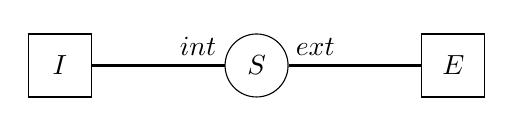
\begin{tikzpicture}[
            node distance={25mm},
            sw/.style = {draw, circle,minimum size=8mm},
            h/.style = {draw, rectangle,minimum size=8mm}
        ]
        \node[h] (i)  {$I$};
        \node[sw] (s) [right of=i]  {$S$};
        \node[h] (e)  [right of=s] {$E$};
        \draw [thick] (i)  -- node[above,pos=0.8]{$int$} (s);
        \draw [thick] (s) -- node[above,pos=0.2]{$ext$} (e);
    \end{tikzpicture}
    \caption{مثال دیوار آتش}
    \label{fig:dynetkat:firewall}
\end{figure}
در ادامه چگونگی توصیف یک دیوار آتش
\lf{Firewall}
وابسته به حالت
\lf{Stateful}
با استفاده از نت‌کت پویا بیان می‌شود.
شبکه‌ی شکل
\ref{fig:dynetkat:firewall}
را در نظر بگیرید.
در این شبکه هدف این است که امکان ارتباط از داخل شبکه به بیرون فراهم باشد ولی امکان ارسال بسته از خارج شبکه ممکن نباشد.
اما زمانی که یک بسته به خارج شبکه ارسال شد، دیوار آتش باید اجازه‌ی عبور بسته‌ها از بیرون را بدهد تا پاسخ بسته‌ها دریافت شوند.
برای توصیف این شبکه می‌توان از عبارت نت‌کت پویای زیر استفاده کرد:
\begin{align*}
    Host  \triangleq   & secConReq!1;Host \oplus secConEnd!1;Host        \\
    Switch \triangleq  & (port = int) \cdot (port \la ext);Switch \oplus \\
                       & (port = ext)\cdot 0 ; Switch \oplus             \\
                       & secConReq?1;Switch'                             \\
    Switch' \triangleq & (port =int) \cdot (port \la ext);Switch' \oplus \\
                       & (port=ext)\cdot(port\la int);Switch' \oplus     \\
                       & secConEnd?1;Switch                              \\
    Init \triangleq    & Host \parallel Switch
\end{align*}
در این توصیف عملیات 
$secConReq$
برای شروع ارتباط امن و
$secConEnd$
برای خاتمه‌ی ارتباط امن در نظر گرفته شده‌است.
بنابراین برنامه‌ی سوییچ پس از دریافت پیام برای شروع ارتباط امن تبدیل به برنامه‌ی 
$Switch'$
می‌شود که در آن اجازه‌ی ارسال بسته از پورت خارجی به پورت داخلی را دارد.
پس از دریافت پیام برای خاتمه‌ی ارتباط امن، برنامه به حالت اولیه‌ی خود بر می‌گردد و دوباره تمامی بسته‌های ورودی از پورت خارجی را رها می‌کند.
در نهایت رفتار کل شبکه با استفاده از ترکیب موازی یک هاست و یک سوییچ در حالت اولیه خود توصیف می‌شود.
\begin{figure}[ht]
    \centerline{\includegraphics[width=0.8\textwidth]{mine/firewall-lts.png}}
    \caption{سیستم انتقال برچسب‌دار برای شبکه‌ی دیوار آتش}
    \label{fig:dynetkat:lts}
\end{figure}
نمودار نمایش داده شده در شکل
\ref{fig:dynetkat:lts}
سیستم انتقال برچسب‌دار
\lf{Labeled Transition System}
این شبکه‌ را در حالتی که یک بسته روی پورت ورودی و یک بسته روی پورت خروجی شبکه وجود دارد نشان می‌دهد.
همانطور که در نمودار مشخص است، عملیات
$(\sigma_e,\sigma_i)$
که به معنای ارسال بسته از پورت ورودی به پورت خروجی است تنها در قسمتی از این سیستم انتقال قابل دسترسی است که پیش از آن یکی از عملیات‌های
$SCR?1$
یا
$rcfg(SCR,1)$
انجام شده باشند.
بنابراین در این حالت شبکه تنها در صورتی که بسته خارجی را به داخل ارسال می‌کند که پیش از آن پیام آغاز ارتباط امن دریافت کرده‌ باشد.
